\documentclass[a4paper, 12pt]{jarticle}
\usepackage[dvipdfmx]{graphicx}
\usepackage{amsmath, amsthm, url}
\title{私のための「頻度論」統計学入門}
\author{}
\西暦
\begin{document}
\maketitle
\tableofcontents

\theoremstyle{definition}
\newtheorem{theorem}{定理}
\newtheorem*{theorem*}{定理}
\newtheorem{definition}[theorem]{定義}
\newtheorem*{definition*}{定義}

\newcommand{\KL}{D_{\mathrm KL}}

\section*{記法}

$\log(x)$ は自然対数を表す.

\section{確率の話}
ここでは主に大数の法則, 中心極限定理, カルバック・ライブラ情報量について勉強する.

\subsection{大数の法則}

いろいろな本に書いてある. いまそれらを勉強しているところなので,  後で書く.

\subsection{中心極限定理}

中心極限定理の証明には, 特性関数やモーメント母関数を使うことが多い. 

テイラー展開を使ったより簡単な証明が, 黒木 (2017) にある. 

\subsection{カルバック・ライブラ情報量}
統計的推測のために重要な役割を果たす量の1つにカルバック・ライブラ情報量がある.
カルバック・ライブラ情報量$\KL(p\|q)$は離散型の確率関数$p(x)$と$q(x)$に対しては, 
\begin{align}
\KL(p\|q) = -\sum_{x} p(x) \log \frac{q(x)}{p(x)}
\end{align}
連続型の確率密度関数$p(x)$と$q(x)$に対しては, 
\begin{align}
\KL(p\|q) = -\int p(x) \log \frac{q(x)}{p(x)} \, dx
\end{align}
と定義される. 
赤池(1980)に習って, カルバック・ライブラ情報量の直感的な意味を考える. 結論を先取りすると, カルバック・ライブラ情報量は「サンプルを生成した分布が $q(x)$ のとき, 経験分布がほぼ $p(x)$ となる確率の対数のサンプルサイズ分の 1 の符号反転」と解釈できる. このカギカッコの中身の意味がわかるようになることがこの節の目標である.

状態 $i=1,\ldots,M$ がそれぞれ $q_i$ の確率で生起する分布と, 状態 $i=1,\ldots,M$ がそれぞれ $p_i$ の確率で生起する分布を考える. この分布からのサンプルを $N$ 個観測して、状態 $i=1,\ldots,M$ が生起した回数をそれぞれ $N_1,\ldots,N_M$ とする. $ N=\sum_{i=1}^{M}N_i$ である. 
$N_1,\ldots,N_M$ のような観測が得られる確率は,
\begin{align}
W=\frac{N!}{N_1! \cdots N_M!}q^{N_1}_1 \cdots q^{N_M}_M
\end{align}
と表せる. (このような分布は多項分布と呼ばれる.)

ここでスターリングの公式
\begin{align}
\log N! \approx N\log N -N
\end{align}
を使って $\log W$ を近似すると
\begin{align}
\log W &\approx (N \log N) - \sum_{i=1}^{M}( N_i \log N_i -N_i) + \sum_i=1^{M} \log q_i \\
&= N \log N - \sum_{i=1}^M N_i (\log N_i - q_i) \\
&= - \sum_{i=1}^M N_i (\log N_i - q_i -\log N ) \\
&= - \sum_{i=1}^M N_i (\log \frac{N_i}{N} - q_i) \\
&= - N \sum_{i=1}^M \frac{N_i}{N} (\log \frac{N_i}{N} - q_i) 
\end{align}
と整理できる.
$p_i = N_i/N$ とおくと
\begin{align}
\log W \approx -N\sum_{i=1}^{M}p_i \log\frac{p_i}{q_i}
\end{align}
という結果を得る.

あらためて考えると $p_i = N_i/N$  は経験的に推定された確率と解釈できる.
$q_i$ は真の確率であったことを思い出すと、$W$ はサンプルを生成した真の分布が $q_i$ のときに $p_i$ のように振る舞う確率と解釈できる. 
$\log W$を $N$ で割り, 符号を反転させると, $-\sum_{i=1}^{M} p_i \log {\frac {q_i}{p_i}}$ となる.
この量は「母集団分布が $q_i$ のとき経験分布がほぼ $p_i$ となる確率の対数のサンプルサイズ分の 1 の符号反転」と解釈できる.

カルバック・ライブラ情報量は次の性質を満たすため, 分布の近さを測る指標となる. 
\begin{align}
\KL(p\|q) \ge 0,
\end{align}
かつ, $\KL(p\|q) = 0$となるのは $p(x)=q(x)$のときに限られる.

\paragraph{注意.}
定義をよく見ればわかるように, カルバック・ライブラ情報量では $\KL(p\|q) =\KL(q\|p)$ は成り立たない. 

\subsection{シミュレーション}

サンプルサイズが増えれば増えるほど正規分布でないことがはっきりしてくる.

\section{最尤法}
本節では最尤法と呼ばれる方法の性質について述べる. これについて理解するために, フィッシャー情報量と呼ばれる量が重要になるため, 先にフィッシャー情報量についての性質を述べる. 

\subsection{パラメータが1つの場合}

\subsubsection{スコア関数とフィッシャー情報量}
パラメータ $\theta$ を持つ確率(密度)関数 $p(x|\theta_0)$ について, スコア関数 $S(\theta)$ を次のように定義する. 
\begin{align}
S(\theta) = \frac{d}{d\theta}\log p(x | \theta). 
\end{align}
スコア関数の $p(x|\theta)$ による平均は 0 である.  
\begin{align}
&\int_{-\infty}^{\infty} \frac{d}{d\theta}\log p(x | \theta) p(x|\theta)\, dx \\
&= \int_{-\infty}^{\infty} \frac{\frac{d}{d\theta}p(x | \theta)}{p(x | \theta)} p(x|\theta) \, dx \\
&=\int_{-\infty}^{\infty} \frac{d}{d\theta}p(x | \theta)\, dx \\
&=  \frac{d}{d\theta} \int_{-\infty}^{\infty} p(x | \theta)\, dx\\
&= 0.
\end{align}
従い, スコア関数の分散はスコア関数の2乗の平均に等しい.

フィッシャー情報量を
\begin{align}
I(\theta)=-\int^{\infty}_{-\infty}\left(\frac{d^2}{d \theta^2} \log p(x_i | \theta)\right) p(x|\theta) \, dx
\end{align}
と定義すると, 
\begin{align}
I(\theta)&=-\int^{\infty}_{-\infty}\frac{d}{d \theta} \left(\left(\frac{\frac{d}{d\theta} p(x_i | \theta)}{p(x|\theta)}\right) p(x|\theta) \right) \, dx \\
&=-\int^{\infty}_{-\infty}\left(\left(\frac{\frac{d^2}{d\theta^2} p(x_i | \theta)}{p(x|\theta)} - \frac{ ( \frac{d}{d\theta} p(x_i | \theta))^2}{p(x|\theta)^2 }\right) p(x|\theta) \right) \, dx \\
&=-\int^{\infty}_{-\infty}\left(\frac{\frac{d^2}{d\theta^2} p(x_i | \theta)}{p(x|\theta)}\right) p(x|\theta) \, dx +\int^{\infty}_{-\infty}\left( \frac{ ( \frac{d}{d\theta} p(x_i | \theta))^2}{p(x|\theta)^2 }\right) p(x|\theta) \, dx
\end{align}
スコア関数のときと同様, 第1項は消える. 
第2項は
\begin{align}
\int^{\infty}_{-\infty}\left(\frac{d}{d\theta} \log p(x | \theta)\right)^2 p(x|\theta) \, dx 
\end{align}
と等しい. これはスコア関数の2乗の平均になっている. 
すなわち, スコア関数の分散はフィッシャー情報行列と等しいことがわかった. 

\subsubsection{最尤推定量の性質}
\label{secPropertyMLE}
サンプル $x_i$ ($i=1,\ldots n$) が, 独立に同一の確率(密度)関数 $p(x|\theta_0)$ を持つ分布から得られたとする\footnote{ 「独立に同一の確率分布に従う」ことを i.i.d. (independent and identically distributed) と略すことがある.}. ここで $\theta$ は確率(密度)関数のパラメータである\footnote{このパラメータのことを母数と呼ぶことがあるが, 母数という語は誤解を招くことが多いので, 本稿ではあまりつかわない.}.  
このようなデータに対し, 統計モデル $p(x|\theta)$ を考え, 未知パラメータの $\theta$ を推定したい.

まず, 次の対数尤度比関数 $l_n(\theta)$ を考える. 
\begin{align}
l_n(\theta) = \log \left( \frac{\prod_{i=1}^{n}p(x_i|\theta)}{\prod_{i=1}^{n}p(x_i|\theta_0)} \right) = \sum_{i=1}^{n}\log \left(\frac{\log p(x_i| \theta)}{\log p(x_i| \theta_0)}\right).
\end{align}
これをサンプルサイズ(標本の大きさ) $n$ で割ると大数の法則により, 
\begin{align}
\lim_{n\to \infty} l_n(\theta)/n &= \int_{-\infty}^{\infty} p(x|\theta_0)\log \left(\frac{p(x| \theta)}{ p(x| \theta_0)}\right) \, dx
\end{align}
となる. 右辺はサンプルを生成した分布と, 統計モデルのカルバック・ライブラ情報量の$-1$倍となっている. そのため, サンプルを生成した分布と統計モデルのカルバック・ライブラ情報量を最小にするためには $l_n(\theta)$ を最大にすればよいことが予想される.
$l_n(\theta)$ の式を少し変形する. 
\begin{align}
 l_n(\theta)= \sum_{i=1}^{n}\log p(x| \theta) \, dx -  \sum_{i=1}^{n}\log p(x_i| \theta_0)\, dx.
 \label{eqln}
\end{align}
右辺第2項は, サンプルを生成した分布のみによって定まる量であり, 統計モデルのパラメータ $\theta$ の選び方に依存しない. 
よって, $l_n(\theta)$ を最大にするためには, 第1項を最大にする $\theta$ を探せばよい. これが最尤法と呼ばれる推定方法のアイデアである.

$l_n(\theta)$ を最大化する $\theta$ は, 確率変数としてどのような振る舞いをするだろうか. 
そのことを調べるために, テイラー展開を使う. 
関数 $f(x)$ の $x_0$のまわりでのテイラー展開は, 
\begin{align}
f(x)= f(x_0) +f'(x_0) (x-x_0) + \frac{1}{2}f''(x_0)(x-x_0)^2 + \cdots 
\end{align}
であった. テイラー展開についてよく知らない場合は(なにかいい本)を参考にするとよい. 
$l_n(\theta)$ の $\theta_0$ の周りでのテイラー展開は, 
\begin{align}
l_n(\theta)= l_n(\theta_0) +l_n'(\theta_0) (\theta-\theta_0) + \frac{1}{2}l_n''(\theta_0)(\theta-\theta_0)^2 + \cdots 
\end{align}
である. 
$h/\sqrt{n}=\theta-\theta_0$と置くと, 
\begin{align}
l_n(\theta_0 + h/\sqrt{n})= l_n(\theta_0) +\frac{l_n'(\theta_0)}{\sqrt{n}}h+ \frac{1}{2n}l_n''(\theta_0)h^2 + \cdots 
\end{align}
となる. $h$ を $\sqrt{n}$ で割ったのは後の計算の便宜のためである.
$l_n(\theta_0) = \log{1} =0$ であるから, 
\begin{align}
l_n(\theta _0+ h/\sqrt{n})= \frac{l_n'(\theta_0)}{\sqrt{n}}h+ \frac{1}{2n}l_n''(\theta_0)h^2 + O(1/\sqrt{n})
\end{align}
と書ける.  ここで $O$ はランダウの記号である. ランダウの記号については(なにかいい本)を参考にするとよい. 
$l_n(\theta)$ の定義に戻ると, 
\begin{align}
&l_n(\theta_0 + h/\sqrt{n})  \nonumber \\
&\approx \frac{1}{\sqrt{n}} \left[\sum_{i=1}^{n} \left( \frac{d}{d \theta}  \log p(x_i | \theta) |_{\theta=\theta_0} \right)\right] h+ \frac{1}{2n}\left[  \sum_{i=1}^{n}\left(\frac{d^2}{d \theta^2} \log p(x_i | \theta)|_{\theta=\theta_0}\right)\right] h^2. 
\end{align}
スコア関数とフィッシャー情報行列についての性質を思い出すと, 大数の法則と中心極限定理より $n$ が十分大きいとき,  標準正規分布に従う確率変数 $Z$ を用いて, 
\begin{align}
l_n(\theta_0 + h/\sqrt{n}) &\approx Z \sqrt{I(\theta_0)} h  - \frac{I(\theta_0) h^2}{2} \\
&= -\frac{I(\theta_0)}{2}\left(h - \frac{Z}{\sqrt{I(\theta_0)}}\right)^2 + \frac{Z^2}{2}
\end{align}
という近似が成り立つ. $\theta=\theta_0 + h/\sqrt{n}$であったので,
\begin{align}
l_n(\theta)&= -\frac{I(\theta_0)}{2}\left(\sqrt{n}(\theta - \theta_0 )- \frac{Z}{\sqrt{I(\theta_0)}}\right)^2 + \frac{Z^2}{2}
\label{reslik}
\end{align}
右辺は2次関数であり, $\sqrt{n}(\theta - \theta_0) = Z/\sqrt{I(\theta_0)}$ のとき最大になる.
よって $l_n(\theta)$ を最大にするよう $\theta$ を決めると, $\sqrt{n}(\theta - \theta_0)$ は平均 0, 分散 $I(\theta_0)^{-1}$ の正規分布に従う.
これが最尤法の基礎である.
最尤法により推定された $\theta$ を最尤推定量と呼ぶ. 最尤推定量は確率変数であるから, サンプルを生成した分布のパラメータそのものではない. 
そこで最尤推定量は $\hat \theta$ などの記号を用いて, パラメータと区別する. 

より直感的に述べると, 最尤推定量 $\hat \theta$ はサンプルサイズが十分大きいとき, 平均 $\theta_0$, 分散 $I(\theta_0)^{-1}/n$ の正規分布に従うということである. 

\paragraph{最尤推定の手順.} 
\begin{enumerate}
\item データ$X$を生成した分布に対し, 同時確率(密度)関数$p(X|\theta)$を適当に与える. 
\item $p(X|\theta)$ を $\theta$ の関数とみて, $p(X|\theta)$ を最大化する $\theta$ をなんらかの方法で探し, 推定量とする.
\end{enumerate}
$p(X|\theta)$ を $\theta$ の関数とみるときは尤度関数と呼ばれる. その対数をとったもの $\log p(X|\theta)$ を対数尤度関数と呼ぶ. 対数を取ることは多くの場合, 計算をとても便利にする. 

\subsubsection{例題}
まずは二項分布, ポアソン分布, 指数分布などで練習すると良い.

\subsection{パラメータが複数の場合}

対象とする確率分布がパラメータを複数持つ場合, 多変数のテイラー展開を用いることで, パラメータが1つの場合と同様の議論を展開することができる. 



\subsection{間違ったモデルで最尤推定すること}
サンプルを生成した分布と統計モデルが, パラメータのとり方によっては厳密に一致するとき, サンプルを生成した分布が統計モデルによって実現可能であるという. 
上記ではサンプルを生成した分布が統計モデルによって実現可能である場合を論じた. しかし, 現実にはサンプルを生成した分布は未知であり, 統計モデルは分析者が設定する. そのため, 統計モデルによって, サンプルを生成した分布が実現可能かどうかはわからない. 

最尤推定は真の分布とモデルの間のカルバック・ライブラ情報量を経験的に最小化する方法であったことを思い出すと, 最尤法は「間違ったモデル」を選んでも, 選んだ範囲内で(カルバック・ライブラ情報量の意味で)適切な推定を行うことが予想される. 

しかし, このことを一般的に保証するような定理は今のところないと思う. 

\subsubsection{例題}
サンプルを生成した分布が確率密度関数
\begin{align}
g(x) = \frac{1}{6}x^3 exp(-x)
\end{align}
を持つとする. (この分布はガンマ分布と呼ばれる分布の一例である.)
統計モデルを正規分布とする. 

サンプルを生成した分布と統計モデルの間のカルバック・ライブラ情報量は, 
 \begin{align}
 E_g (-\log6+3\log X-X)-\frac{1}{2}E_g\{\log(2\pi \sigma^2)) + \frac{(X-\mu)^2}{\sigma^2}\}
 \end{align}
 である. ここで, $E_g[X] = \int xg(x)\, dx$.
 
(途中計算は省略して)

$\hat \mu=4$, $\hat \sigma^2=4$で, 真の分布とモデルの間のカルバック・ライブラ情報量は最小となる. 
R を使って最尤推定のシミュレーションをしてみる.
その結果を図\ref{figWrongmodel} に示す.

\begin{figure}[htbp]
 \begin{minipage}{0.5\hsize}
  \begin{center}
   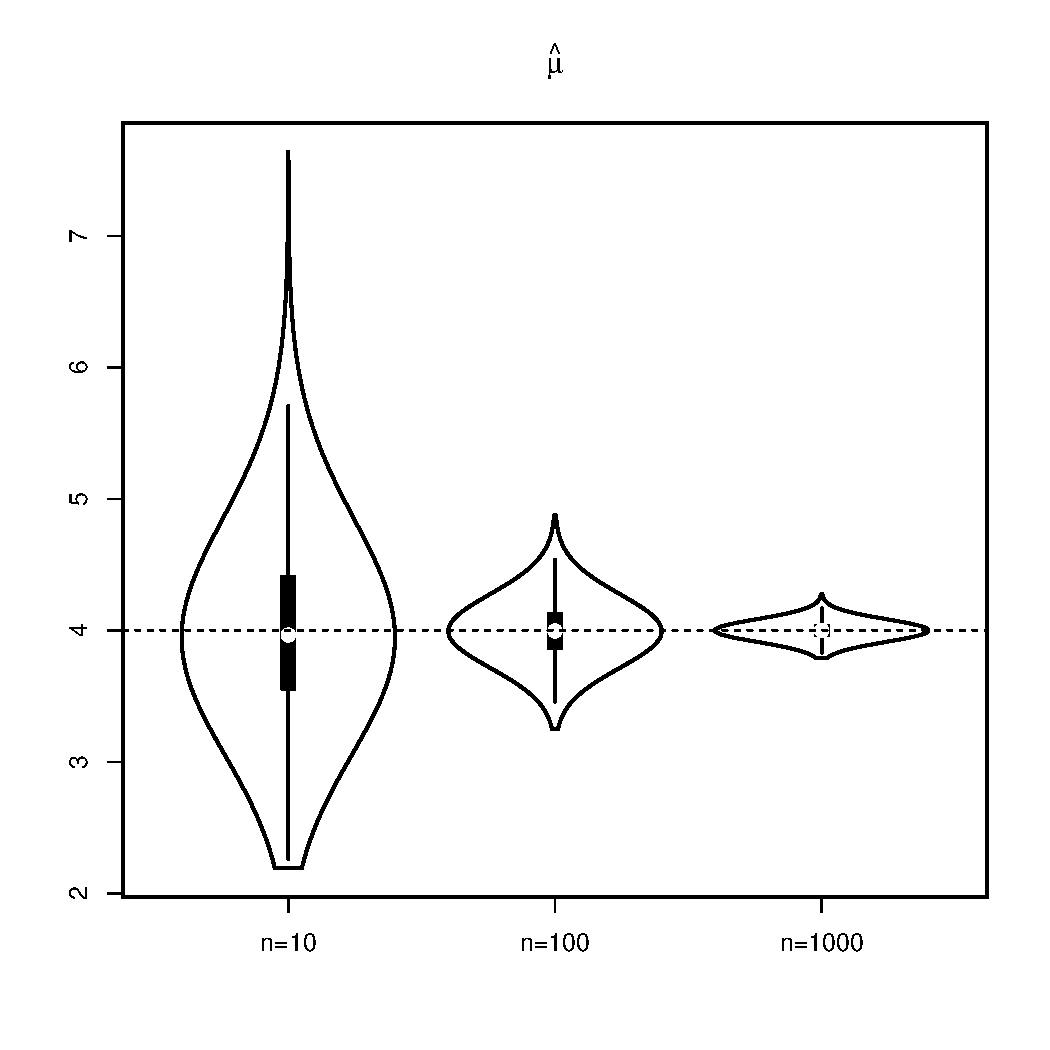
\includegraphics[width=70mm]{img/wrongmodel_mu.pdf}
  \end{center}
 \end{minipage}
 \begin{minipage}{0.5\hsize}
  \begin{center}
   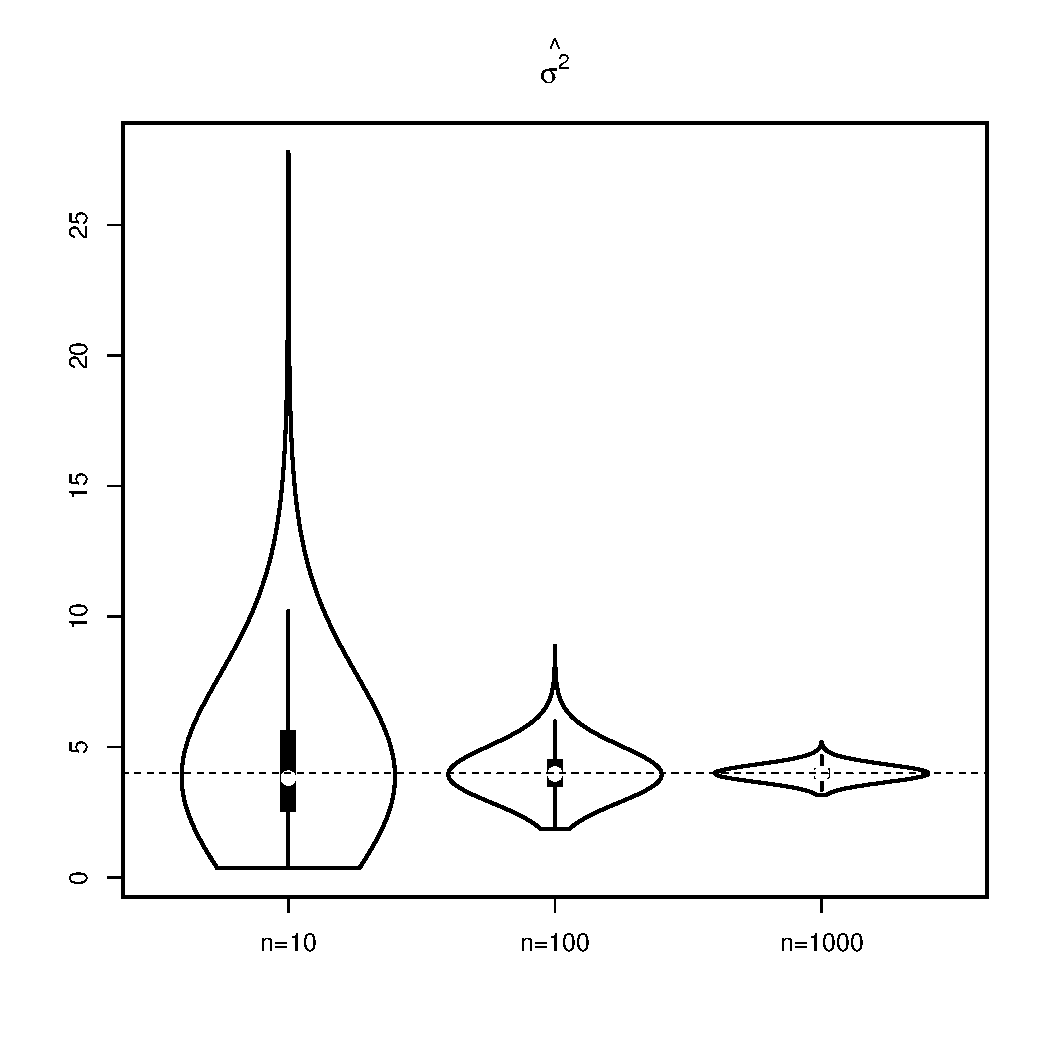
\includegraphics[width=70mm]{img/wrongmodel_sigma2.pdf}
  \end{center}
 \end{minipage}
   \caption{最尤推定量の分布を示すバイオリンプロット. $n$ はサンプルサイズ.}
  \label{figWrongmodel}
\end{figure}

図\ref{figWrongmodel} からは推定量が, カルバック・ライブラ情報量が最小となる点を中心に分布し, サンプルサイズが大きくなるに従って分散が小さくなる様子が伺える.
しかし, この例にどれだけ一般性があるかはわからない.

この例は Pawitan (2001) にあったものを参照している.

シミュレーションに用いたスクリプトは R フォルダにある wrogmodel.R である.



\section{カイ二乗分布を使った検定}

$Z$ を標準正規分布に従う確率変数とすると $Z^2$ は自由度1のカイ二乗分布に従う. 
自由度 $r$ のカイ二乗分布とは, 以下の確率密度関数を持つ分布である. 
\begin{align}
f(x) = \frac{1}{2^{r/2}\Gamma(r/2)}x^{r/2-1}\exp(-x/2).
\end{align}

また $Z_1, Z_2, \ldots, Z_r$ が独立でそれぞれ標準正規分布に従うとき, $Z_1^2+ Z_2^2+ \cdots +Z_r^2$ は自由度 $r$ のカイ二乗分布に従う. 

(\ref{reslik}) 式の結果を思い出すと, 対数尤度比関数 $l_n(\theta)$ が最大になるとき, その最大値の2倍は $Z^2$ であった. このことから, 尤度関数を用いた検定にカイ二乗分布が使えそうなことがわかる. 

\subsection{Wilks の定理}
\label{secWilks}
あとで書く. 

\subsection{$2 \times 2$分割表の独立性の検定}
様々な分野で表\ref{2by2}のようなカウントデータの表を考えることがある. このとき, 各行(暴露の有無)と各列(疾病の有無)は独立か, という問いに関心があることが多い. 
ここでいう独立とは, ...

\begin{table}[htbp]
\centering
\caption{$2 \times 2$分割表.}
\label{2by2}
\begin{tabular}{l|cc|c}
 & 疾病あり&疾病なし&合計\\
 \hline
 暴露あり&$a_{11}$&$a_{12}$&$N_1$\\
 暴露なし&$a_{21}$&$a_{22}$&$N_2$\\
  \hline
 合計 & $M_1$ & $M_2$ & $N$
\end{tabular}
\end{table}

このようにシンプルな例でも, 統計モデルは複数考えることができる. 以下では, この分割表を$A=(a_{ij})$と表記する. 

\subsection{二項分布モデル}
$a_{i1}$ がそれぞれ独立にパラメータ $q_i$ の二項分布に従うとする.  
$Q=(q_i)$ とおく. 
$A$ が生じる確率$p(A|Q)$は, 
\begin{align}
p(A|Q) = \prod_{i=1}^2 \frac{N_i!}{a_{i1}!a_{i2}!}( q_i^{a_{i1}}(1-q_{i})^{a_{i2}})
\end{align}
とかける.
この場合, $q_i$ の最尤推定量は, $\hat q_{i}=a_{i1}/N_i$ である. 

分割表の各行と各列は独立であるとするモデルを, パラメータが $q_0=q_1=q_2$ という条件を満たしているモデルだとする. 
この場合, $q_0$ の最尤推定量は, $\hat q_{0}=M_1/N$ である.

次にこの2つのモデルの対数尤度比統計量 $G_0$ を考える.
\ref{secWilks}節で述べた通り, $G_0$はサンプルサイズが十分大きいとき, 自由度1のカイ二乗分布に近似的に従う. 
\begin{align}
G_0 =& 2 \left(\sum_{i=1}^2 \left\{ a_{i1}\log(\hat q_i)+ a_{i2}\log(1-\hat q_i)\right\} -\right. \\
&\left.\sum_{i=1}^2 \left\{ a_{i1}\log(\hat q_0) + a_{i2}\log(1-\hat q_0)\right\}\right)\\
&= 2 \left(\sum_{i=1}^2\left\{ a_{i1}\log\frac{\hat q_i}{\hat q_0} + a_{i2}\log\frac{1-\hat q_i}{1-\hat q_0}\right\}\right)
\end{align}
ここで $\hat q_i/\hat q_0 = a_{i1}/(N_iM_i/N)$,  $(1-\hat q_i)/(1-\hat q_0) = a_{i1}/(N_iM_i/N)$ と書ける.
この統計量 $G_0$ を用いた検定を $G$ 検定と呼ぶことがある.
また$a_{ij}$ を観測度数, $N_iM_i/N$ や $N_iM_i/N$ を理論度数と呼ぶことがある.
$2 \times 2$分割表の独立性の検定において, 理論度数を表\ref{2by2theo} のように定めると, 統計量 $G$ は次のようにも書ける.
\begin{align}
G = 2 \left(\sum_{i,j} a_{ij}\log\frac{a_{ij}}{E_ij} \right).
\end{align}
\begin{table}[htbp]
\centering
\caption{$2 \times 2$分割表の独立性の検定における理論度数.}
\label{2by2theo}
\begin{tabular}{l|cc|c}
 & 疾病あり&疾病なし&合計\\
 \hline
 暴露あり&$E_{11} = N_1M_1/N$&$E_{12} = N_1M_2$&$N_1$\\
 暴露なし&$E_{21} = M_1N_2/N $&$E_{22}=M_2N_2/N$&$N_2$\\
  \hline
 合計 & $M_1$ & $M_2$ & $N$
\end{tabular}
\end{table}

ところで, $\log (1+x)$ を0のまわりでテイラー展開することで次の式が成り立つ. 
\begin{align}
(1+x) \log (1+x) &= (1+x)\left(x-\frac{x^2}{2} + O(x^3)\right) \\
& = x + \frac{x^2}{2} +  O(x^3)
\end{align}
2つめの等号において, かっこを展開すると $x^3$ についての項が出てくるが, $O(x^3)$ に吸収される.

この式を用いると, 統計量 $G$ の式は, 以下のように近似できる.
\begin{align}
&2 \left(\sum_{i,j} a_{ij}\log\frac{a_{ij}}{E_ij} \right)\\
&=2 \left(\sum_{i,j} E_{ij} \left(1+ \frac{a_{ij}-E_{ij}}{E_{ij}}\right)\log\left(1+ \frac{a_{ij}-E_{ij}}{E_ij} \right)\right)\\
&\approx 2 \left(\sum_{i,j} E_{ij}\left(  \frac{a_{ij}-E_{ij}}{E_{ij}}- \frac{(a_{ij}-E_{ij})^2}{E_{ij}^2} \right)\right) \\
&= 2 \left(\sum_{i,j} \frac{(a_{ij}-E_{ij})^2}{E_{ij}} \right).
\end{align}
最後の等号においては, $\sum_{i,j} E_{ij} =\sum_{i,j} a_{ij} = N$ を用いた.
この統計量を$\chi^2_0$とおく. 
$\chi^2_0$は$G_0$とサンプルサイズが十分大きいとき等しい.
すなわち, $\chi^2_0$ はサンプルサイズが自由度1のカイ二乗分布に近似的に従う.

単にカイ二乗検定というときは, この $\chi^2_0$ 統計量を用いた検定を指すことが多い. 

ではカイ二乗検定の手順を具体的に示そう. 

\paragraph{カイ二乗検定の手順.}
データから求めた検定統計量(この場合$G_0$や$\chi^2_0$)以上の値が, 自由度1のカイ二乗分布から出る確率を調べる. その調べた確率をp値と呼ぶ.

p値が小さすぎるとき, 分割表の各行と各列は独立でないと判断する.

どの程度の確率であれば, 小さすぎると判断するかは事前に定めておく. この事前に定めた閾を有意水準と呼ぶ.

\subsubsection{ポアソン分布モデル}
$\Lambda = (\lambda_{ij})$ を正の実数を成分とする$2 \times 2$行列とする. 
$a_{ij}$ がそれぞれ独立にパラメータ $\lambda_{ij}$ のポアソン分布に従うとすると, $A$ が生じる確率$p(A|\Lambda)$は, 
\begin{align}
p(A|\Lambda) = 
\prod_{i,j} \frac{e^{-\lambda_{ij}} \lambda_{ij}^{a_{ij}}}{a_{ij}!}
\end{align}
と書ける. 
分割表の各行と各列は独立であるとするモデルについては表\ref{2by2theo} との対応を考え, 行についてのパラメータ$\mu$と列についてのパラメータ$\nu$,  観測の総数を規定するパラメータ $\tau$ を用いて, 

\paragraph{注意点.}
統計的仮説検定は確率版背理法と例えられることもあるが, 現実のデータを扱う以上, 背理法のようにすっきりとはいかない. 
具体的にどのような難しさがあるかは \ref{secWaldtest} 節で改めて詳しく述べる. 

\subsubsection{カイ二乗検定のシミュレーション}
$\chi^2_0$は$G_0$とサンプルサイズが十分大きいとき等しいと述べたが, サンプルサイズが小さいときには大きく性質がことなる.
どの程度のサンプルサイズのとき, どのような性質を持つかを調べるには, コンピューターを使ってシミュレーションするのが早い. 

本当は分割表の各行と各列が独立であるときに, 分割表の各行と各列が独立でないと誤って判断する確率を $\alpha$ エラーと呼ぶ.
本当は分割表の各行と各列が独立でないときに, 分割表の各行と各列が独立でないと正しく判断する確率を検出力(power)と呼ぶ.

よい仮説検定の第1条件は, まずなによりも$\alpha$エラーをコントロールできること, 第2の条件は検出力が高いことである. 

$G$ 検定はサンプルサイズの小さいとき, 実際の$\alpha$エラーが名目上の有意水準を上回ることが多い. 
カイ二乗検定は概ね正確な $p$ 値を与えることが多い.

\paragraph{注意点. } 本説の議論は, 一般の $r \times c$ 分割表にも拡張できる. しかし, $r \times c$ 分割表をカイ二乗検定で分析するのは, 私があまり好きではないので, 本稿では扱わない.

$r$ と $c$ が 2より大きいとき, $r \times c$ 分割表の独立性のカイ二乗検定では, 行と列が独立でないことは言えても, どの行とどの列に特に大きな関係があるかはわからない. 

そこでカイ二乗検定を行った後に, 残差分析と呼ばれる分析を行うことがある. しかし, このように検定を何段階も行うことの, 多重比較のような問題を考え出すと話がややこしくなるように思う.  

連続量を大, 中, 小のように分けて表にした場合は, 元の連続量に対する統計モデルを考えたほうがいいように思う. また, 順序尺度の量を集計した場合は, 順序尺度に対する統計モデルを考えたほうがいいように思う. 
順序尺度に対する統計モデルは, \ref{secCata} 節で扱う予定である. 

\section{ワルド検定とワルド信頼区間}
\subsection{ワルド検定}
\label{secWaldtest}
\ref{secPropertyMLE} 節で述べた通り, サンプルサイズが十分大きいとき, 最尤推定量は平均 $\theta$, 分散 $I(\theta)^{-1}/n$ の正規分布で近似できた. ここで $I(\theta)$ はフィッシャー情報量である. 
しかし, 仮に統計モデルとしてデータを生成した分布を実現可能な分布を選んだとしても\footnote{一般には, データを生成した分布を実現可能な分布を選ぶということはとても難しい. その方法はわかっていない. }, 正しいパラメータ $\theta$ は不明であり, 解析的な期待値の計算も難しいことが多い. 
 
そこでサンプル $x_i$ ($i=1,\ldots,n$) が得られたときの, 統計モデル $p(x|\theta)$ の観測情報量 $I_o(\theta)$ を次のように定義する.
\begin{align}
I_o(\theta)=\frac{1}{n}\sum_{i=1}^{n} \frac{\partial^2}{\partial \theta^2}\log p(x_i|\theta).
\end{align}
サンプルサイズ$n$が十分大きいとき, $I_o(\theta)$ は $I(\theta)$ に近づく. 
これにより, 最尤推定量は分散 $I_o(\hat \theta)^{-1}/n$ の正規分布で近似できる. 

$\theta$が不明なので, 最尤推定量$\hat \theta$を用いて近似するわけである. このように計算していい根拠は実はよくわからない. ここでいうわからないは, 私個人がわかっていないという意味であり, 統計学的に未解決ということではない. 
 
上記の性質から, ワルド検定統計量 $z_0$ を次のように定義する. 
\begin{align}
z_0=\frac{\hat \theta-\theta_0}{\mathrm{se}(\hat \theta)},
\label{Waldstat}
\end{align}
ここで $\mathrm{se}(\hat \theta) = (nI_o(\theta))^{-1/2}$ とおいた. 

カイ二乗検定の説明ではかなり省略して書いたので, ここで仮説検定の枠組みを説明しなおす.
仮説検定では次のように「仮説」を設定する. 
\begin{align}
H_0:~\theta = \theta_0\\
H_1:~\theta \neq \theta_0\\
 \end{align}
 $H_0$ を帰無仮説, $H_1$ を対立仮説という.
(\ref{Waldstat})式での $\theta_0$ は帰無仮説 $H_0: \theta = \theta_0$ と対応している.
求めた検定統計量 $z_0$ より絶対値の大きい値が出る確率(p値)を標準正規分布から求め, p値があらかじめ定めた有意水準より小さいとき, 帰無仮説が棄却されたという.
この形の検定を両側検定という. 

一方で仮説を次のように設定することもある. 
\begin{align}
H_0:~\theta = \theta_0\\
H_1:~\theta > \theta_0\\
 \end{align}
 この場合, $z_0$ より大きい値が出る確率(p値)を標準正規分布から求め, p値があらかじめ定めた有意水準より小さいとき, 帰無仮説が棄却されたという.
この形の検定を片側検定という. 

片側検定の場合, 帰無仮説を$\theta \le \theta_0$ と書きたくなるかもしれないが, 仮説検定では帰無分布(帰無仮説のもとで検定統計量の従う分布)が1つに定まらないと, 計算ができないので, $H_0:~\theta = \theta_0$ という書き方で正しい.

対立仮説を $H_1:~\theta < \theta_0$ と設定しても構わない. その場合は$z_0$ より小さい値が出る確率をp値とする.

\paragraph{注意点.} 
統計的仮説検定は確率版背理法と例えられることもあるが, 現実のデータを扱う以上, 背理法のようにすっきりとはいかない. 
帰無仮説が棄却された場合であっても, $\theta = \theta_0$か$\theta \neq \theta_0$かという, はっきりとした2値的な判断をすることは難しい. 

統計モデルがサンプルを生成した分布からかけ離れていた場合にも, 帰無仮説は棄却されやすくなる. 
例えば独立同分布の仮定というのも, 統計モデリングの一環である. 
統計モデルにおける独立同分布は, 現実の世界でのランダムサンプリングに対応すると思われる. 

\subsection{ワルド信頼区間}
$100(1-\alpha)$\% ワルド信頼区間を次のように定義する.
\begin{align}
[\hat \theta - \mathrm{se}(\hat \theta)z_{\alpha/2}, \hat \theta +  \mathrm{se}(\hat \theta)z_{\alpha/2}]
\label{Waldstat}
\end{align}
ここで $z_{\alpha}$ は標準正規分布の累積分布関数の取る値が $\alpha$ になる点を指している.
これはワルド検定において, $\theta_0$ を動かしたとき, 有意水準 $\alpha$ で帰無仮説が棄却されない範囲を求めている. 

統計モデルによってデータを生成した分布が実現可能であり, サンプルサイズが十分に大きいとき, ワルド信頼区間は次の性質を満たすことが期待される. 
\begin{align}
\Pr[\hat \theta - \mathrm{se}(\hat \theta)z_{\alpha/2} \le \theta \le \hat \theta +  \mathrm{se}(\hat \theta)z_{\alpha/2}] \ge 1-\alpha.
\end{align}
伝統的な統計学の教科書では, この性質 
\begin{align}
\Pr[T_1 \le \theta\le T_2] \ge 1-\alpha
\label{CI}
\end{align}
を満たす $[T_1, T_2]$ を信頼区間と呼ぶ, と定義している場合もある. 
しかし, 信頼区間の作り方は統計モデルに依存するため, 現実の場合, 求めた信頼区間が上記の性質をみたしているかはわからない. 

そこで, 両側検定を行ったときに帰無仮説 $\theta = \theta_0$ が棄却されない $\theta_0$ の範囲のことを信頼区間と呼ぶ, と定義するほうが明快だと思う.

統計モデルによってデータを生成した分布が実現可能なときの $\Pr[T_1 \le \theta\le T_2]$ を被覆確率(covarage probability)という.
被覆確率を計算するためには, コンピューターを使ってシミュレーションを行うのが一般的である.
 
また信頼区間について, 多くの伝統的な統計学の教科書では, 分布しているのは $\theta$ ではなく $[T_1, T_2]$ だから, $\theta$ が $[T_1, T_2]$ に含まれる確率が $1-\alpha$ であると言ってはいけない, と強調している . 

ではどのように解釈するのかというと, 何度もデータを取り, 信頼区間を作ることを繰り返したとき, 信頼区間が $\theta$ を含んでいる割合が $1-\alpha$ だと述べられる.

しかし, 「信頼区間が $\theta$ を含んでいる」は「$\theta$ が信頼区間に含まれる」と同じ意味であるし, この場合の「割合」は「確率」の言い換えに過ぎない. したがって, このような強調が本質的であるとは私には思えない. 

\section{回帰型の統計モデル}

書くかどうか迷っている. これについては久保(2012)などを読んだほうがいいかもしれない.

\subsection{ロジスティック回帰}

回帰と分類の違いを丁寧に説明する資料もあるが, 私にはそのような区別が本質的であるとは思えない. 

%\subsection{ポアソン回帰}

\paragraph{注意点.} 推定されたパタメータの解釈は意外と難しい部分がある. 
推定されたパラメータが統計的に「有意」になっていたとしても, 統計モデルを少し変えるだけでまったく別の結果が出るということは, 頻繁に起こる. 

\section{モデル選択}

統計学の解説では, 正規分布ならば $t$ 検定, 正規分布でないならばノンパラメトリック検定, ラベルデータが与えらていれば識別モデルを使い, 与えらていなければクラスタリング, ……といった, 複雑なフローチャートを記載してあるものがある. 

このようなフローチャートは現実的にはあまり役に立たないことが多い. 例えば「正規分布ならば $t$ 検定」といっても, データが正規分布であるかどうかはわからない\footnote{むしろ, 現実のデータが都合よく正規分布になっていることはありえないと断言したほうがいいかもしれない}. 

本稿は統計モデルは目的に合わせて自由に選ぶという立場をとる. しかし, 選んだモデルが良いかどうかは別の問題である. 
そこで, 作った統計モデルを評価する方法が重要になる.


\subsection{クロスバリデーション}

\paragraph{注意点.}
ディープラーニングのパッケージなどでは, バリデーション損失を簡単にモニタできるようになっていることが多い. これは便利であるが, 弊害もあると感じている.

例えばバリデーション損失をモニタしながら最適化を行い, そのバリデーション損失をそのまま予測精度として報告した場合, 間接的にバリデーション用のデータにフィットするように最適化を行っているのと同じことが起こる気がしている. 

チューニングパラメータの多いモデルの場合, 理想的には, チューニングパラメータを決めるためのバリデーションデータでチューニングを行い, 最終的な予測精度の評価はまた別のバリデーションデータで行うほうが良いと思う. しかしこの方法ではデータが大量に必要になる. 


\section{いくつかの統計モデルのカタログ}
\label{secCata}

統計モデルの紹介がされている楽しい本に松浦(2016)や須山(2017)がある.
ここではこれらの本に記載されていない統計モデルを紹介する. これにより自分の手で統計モデルを作るということがどのようなことか, その雰囲気の一端を感じてもらいたい. 

\subsection{幾何分布回帰}

あるとき, とあるウェブページのアクセス記録のデータを受け取ったとしよう. 
その一部を抜粋したものが, 表 \ref{tabPageDepth} である.

\begin{table}[ht]
\centering
\caption{pageDepth データ}
\label{tabPageDepth}
\begin{tabular}{rlllr}
  \hline
 pageDepth & userGender & userAgeBracket & userType & sessions \\ 
  \hline
 1 & female & 18-24 & New Visitor & 2996 \\ 
 1 & female & 18-24 & Returning Visitor & 382 \\ 
 1 & female & 25-34 & New Visitor & 3426 \\ 
 1 & female & 25-34 & Returning Visitor & 474 \\ 
 1 & female & 35-44 & New Visitor & 1850 \\ 
 1 & female & 35-44 & Returning Visitor & 218 \\ 
   \hline
\end{tabular}
\end{table}

各列の意味を聞いてみると, pageDepth はそのウェブページから離脱するまでに閲覧したページの数, userGender は性別, userAgeBracket は年齢層, userType は新規訪問者かリピーターかを表し, sessions は訪問ののべ人数だという.

このデータからウェブページをたくさん閲覧しやすい(回遊しやすい)のはどのユーザー層か知りたいとする. 

pageDepth を目的変数として回帰を行えば, このデータセットをうまく要約できそうな気がする. 

研究室の後輩に「回帰ってなにがあるんですか? ポアソン回帰とかロジスティック回帰とか、あとは」と聞かれたことがある. 
その答えはもちろん「いくらでもある」である\footnote{おそらく, このように質問させた事自体が, 私のそれまでの指導がまずかったことを意味している.}. そのモデルが良いかどうかは別の問題として, 好きな分布を使って自由に回帰をしてよい. 

このようなデータに対してはどんな分布を用いるのが適切だろうか.

現象を思い切り単純化して考え, コインの表が出たらページを離脱し, コインの裏が出たらページを離脱するとする. このとき, 表が出る確率を $p$ とすると, はじめて表が出るまでのコイントスの回数 $y$ の分布は, 
\begin{align}
f(y|p) = (1-p)^{y-1} p
\end{align}
で表せる. 
このような分布を幾何分布と呼ぶ. 
幸か不幸か, R の glm には幾何分布を使った回帰が実装されていないようなので, ここでは手作りで幾何分布回帰を行う. 

本解析の場合 $y$ は pageDepth に対応する. 
$p$ は0から1の範囲の値を取るパラメータなので, ロジスティック回帰のときと同様, 逆ロジット変換を利用して, 
\begin{align}
p_n = \frac{1}{1+\exp(-X_n \beta)}
\end{align}
という形で, 回帰構造を持たせることにする.

関数の最小値,または最大値を求めることを最適化という. 
R には optim という最適化用の関数があり, これに対数尤度関数を与えれば, 簡単に最尤法を実行することができる\footnote{ただし, 最適化はいつもうまくいくとは限らない. 関数に極値がいくつもあるような場合, 最適化はたやすく失敗する}. 

R では, 対数尤度関数は次のように書けばよい. 

\begin{verbatim}
  ll <- function(beta,y,X,w){
    logprob <- plogis(X %*% beta,log.p = TRUE)
    logprob2 <- plogis(-X %*% beta,log.p = TRUE)
    -sum(w*((y-1)*logprob2+logprob))
  }
\end{verbatim}

R の optim はデフォルトでは最小値を求めるため, 対数尤度に $-1$ を書けた値を返すように, 関数を定義した. 

optim は次のように使う.
\begin{verbatim}
  optim(ini, fn = ll,
        method = "BFGS",
        y=y,X=X,w=w, hessian = TRUE)
\end{verbatim}
ここで \verb|ini| はパラメータの初期値である. \verb| hessian = TRUE | とすることで, 数値微分による目的関数のヘシアンが求まる. これはサンプルサイズで割る前の観測情報量そのものである. 

当てはめた幾何分布と, 実際のデータを並べてプロットしてみよう(図\ref{fitgeomreg}). 
大きな計算ミスはなさそうである. 

\begin{figure}
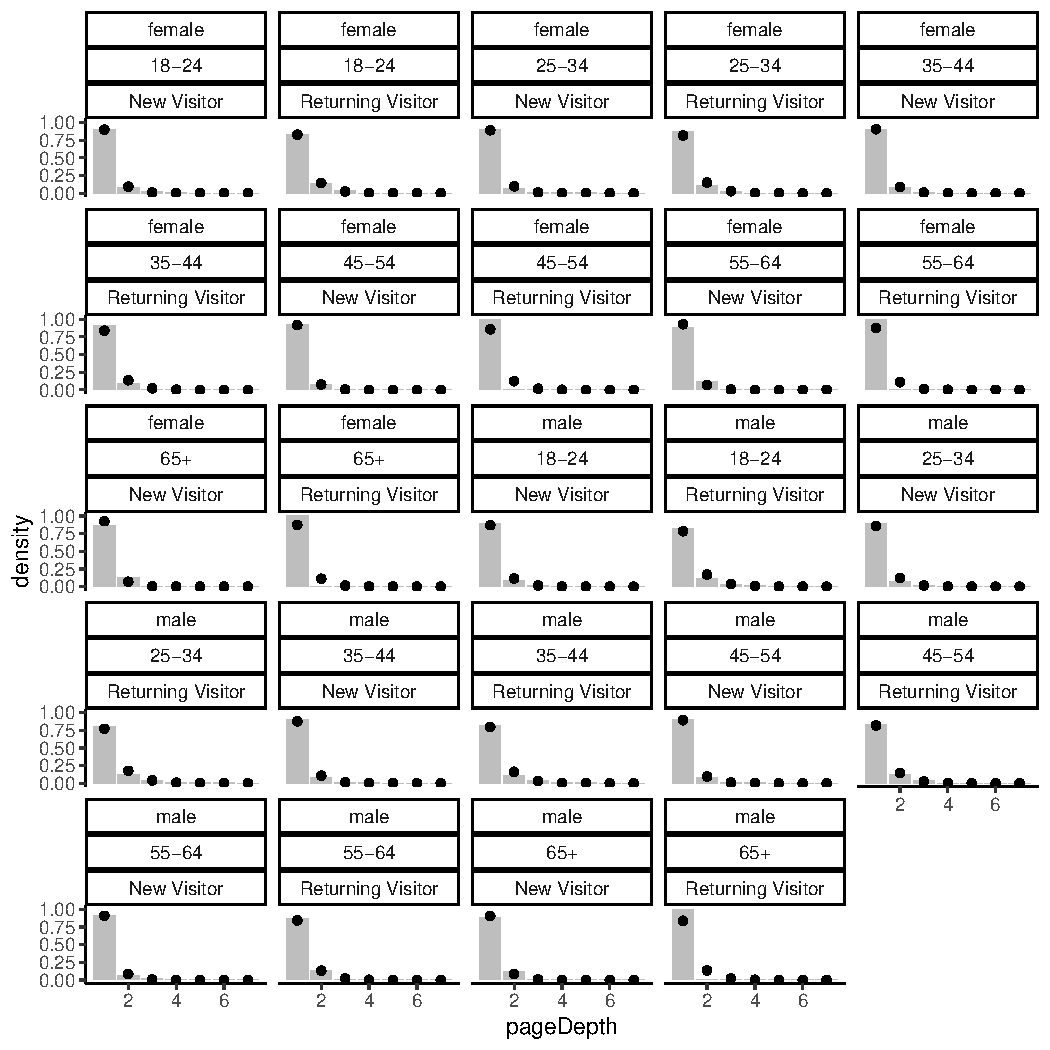
\includegraphics[width=13cm,clip]{./img/fitgeomreg.pdf}
\caption{当てはまりの確認. 棒グラフ: 観測値, 点: 推定値.}
\label{fitgeomreg}
\end{figure}

係数 $\beta$ の推定値と, 観測情報量より計算した2標準誤差のエラーバーをプロットしてみよう(図\ref{coefgeomreg}). 

\begin{figure}
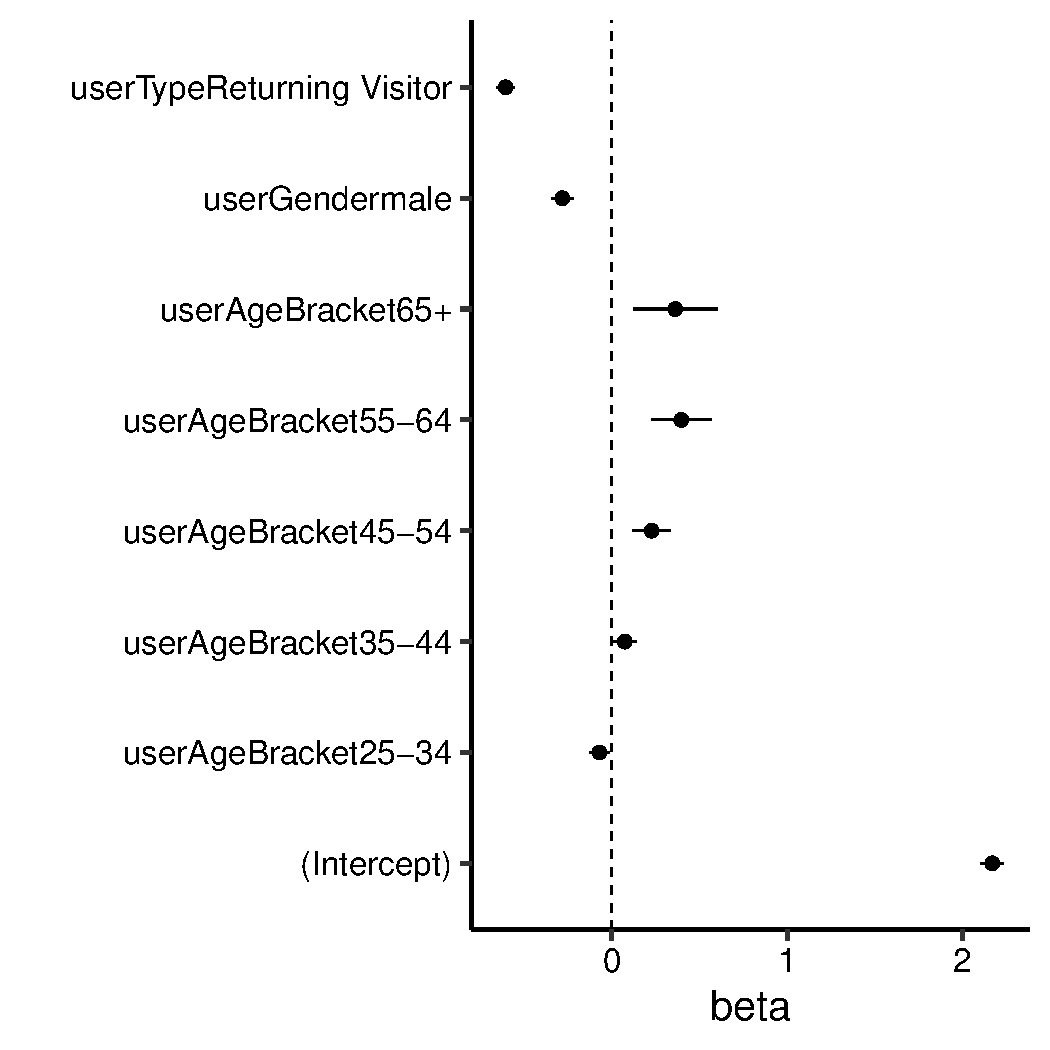
\includegraphics[width=13cm,clip]{./img/coefgeomreg.pdf}
\caption{係数のプロット. バーは2標準誤差.}
\label{coefgeomreg}
\end{figure}

リピーターであるか否かが, サイトを回遊しやすいかどうかに大きく寄与する. 
また, 25-34歳の男性がサイトを回遊しやすい傾向がわかる. 

コードの全体は, R フォルダにある geomreg.R ファイルである. 

\subsection{生存時間分析}

生存時間分析とは死亡や機械の故障といったイベントの発生までの待ち時間を分析することを指す.
特に信頼性工学の分野では, 故障までの待ち時間の統計モデルにワイブル分布が頻繁に利用される.

ワイブル分布はその密度関数を,
\begin{align}
f(y|m,\eta) =
\begin{cases}
\frac{m}{\eta}\left(\frac{y}{\eta}\right)^{m-1}\exp(-(x/\eta)^{m}) & y\geq 0 ,\\
0 & y<0,
\end{cases}
\end{align}
とする分布である.

ワイブル分布は「鎖は弱い輪から切れる」という現象をモデル化したものとして紹介されることが多い.
しかし, 「鎖は弱い輪から切れる」が正しく, 物理現象, 生命現象を反映したものかどうかはわからない.
そこでこの節ではガンマ分布モデルとワイブル分布モデルを実データを用いて比較してみたい.

ガンマ分布はその密度関数を,

とする分布である. 場合によっては $b$ の逆数をとって,

定義されることもあるが, 本質的な違いはないため, 計算上都合のよい方を用いればよい.

R で生存時間分析を行えるパッケージには代表的なものとして surv がある. 
surv で提供される survreg 関数では, デフォルトの分布がワイブル分布に設定されている.
幸か不幸か, R の survreg にはガンマ分布を使った回帰が実装されていないようなので, ここでは手作りでガンマ回帰を行う. 

まず, 次の定理を紹介する. 

\begin{theorem}
$\hat \theta$ が最尤推定量であるとき, 関数 $g(\theta)$ の最尤推定量は $g(\hat \theta)$ である. これを最尤推定量の不変性という.
\end{theorem}
ただし, $g(\theta)$ が1対1の変換になっていないとき, この定理は成り立たない. 

自明な事実を述べたにすぎないと思われると思うので, この定理はなにがうれしいか補足する.

例えば正の値しか取らないパラメータ $\sigma$ を最優推定したいとき, 制約付きの最適化をするのは面倒である. このようなとき, $\sigma=\exp(\rho)$ とおいて, $\rho$ を最尤推定し, $\hat \sigma =\exp(\hat \rho)$ として構わない. 

ワイブル分布もガンマ分布も, パラメータは正の実数値をとるため, この方法を使って最尤推定を行うことができる.

さて, 生存時間分析の特徴は打ち切り\footnote{私の師匠は「打ち切り」でなく, 「打切り」という(JISに則った)表記を好む.}と呼ばれるデータの扱いにある.

観測終了時にまだイベントの発生を経験していないサンプルがあるとき, そのサンプルの観測を右打ち切りされた観測と呼ぶ.  
この場合, データとしては観測終了時点までの待ち時間が記録されることになるが, その記録が持っている情報は, 「本来の寿命は記録された値以上である」ということである.

データセットが右打ち切りを含む場合, 次のような組の変数を用いて記述できる.
$(y_1, d_1), (y_2, d_2), \ldots , (y_n, d_n)$.
ここで, $y_i$ は観測範囲内の待ち時間, $d_i$ はイベントが生起した場合に1, そうでなければ0の値を取る変数である. 

\subsection{比例ハザードモデル}

\subsection{非定常ポアソン過程}
時系列データというと, 等間隔の時点ごとに計測されたデータを思い浮かべることが多い. しかし, イベントの生起がランダムで, イベントの起こった時点だけが記録されていることもある. 

\verb|DSolve[f'[t]==((m/eta^m)*t^(m-1))*(a-f[t]),f[t],t]|

\begin{thebibliography}{4}
\bibitem{Kuroki2017}黒木玄. (2017). 2017-06-04 LindebergのTaylor展開のみを使った中心極限定理の証明.pdf. \url{https://genkuroki.github.io/documents/mathtodon/}.
\bibitem{Akaike1980} 赤池弘次. (1980). エントロピーとモデルの尤度 (〈講座〉物理学周辺の確率統計). 日本物理学会誌, 35(7), 608-614.
\bibitem{Pawitan2001} Pawitan, Y. (2001). \textit{In all likelihood: statistical modelling and inference using likelihood}. Oxford University Press.
\bibitem{Kubo} 久保拓弥. (2012). データ解析のための統計モデリング入門---般化線形モデル・階層ベイズモデル・MCMC. 岩波書店.
\bibitem{Matsuura} 松浦健太郎. (2016) StanとRでベイズ統計モデリング. 共立出版.
\bibitem{Suyama} 須山敦史. (2017) ベイズ推論による機械学習入門. 講談社.
\end{thebibliography}

\end{document}
